\documentclass[tikz]{standalone}
\usetikzlibrary{trees,calc}
\begin{document}
\tikzset{
    every node/.style={
        draw=black,
        thick,
        anchor=west,
        inner sep=2pt,
        minimum size=1pt,
    }
}
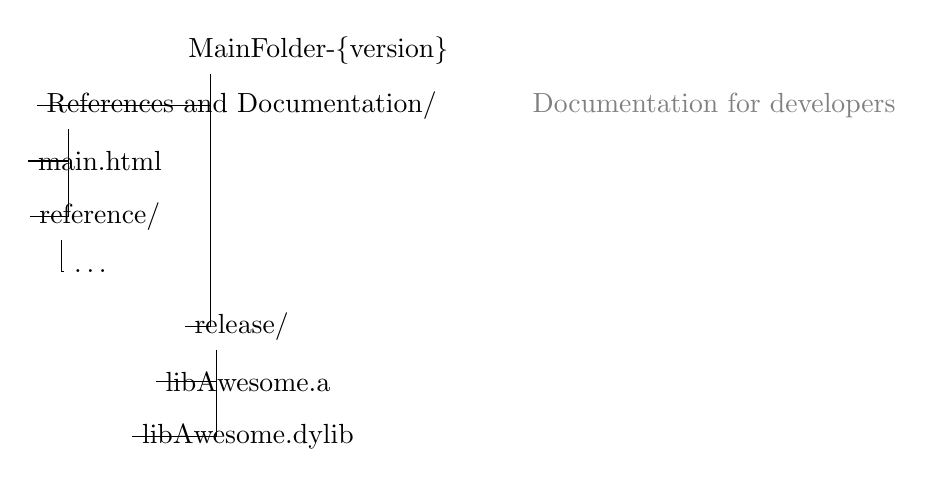
\begin{tikzpicture}[
    grow via three points={
        one child at (0.8,-0.7) and two children at (0.8,-0.7) and (0.8,-1.4)
    },
    edge from parent path={
        ($(\tikzparentnode\tikzparentanchor)+(.4cm,0pt)$) |- (\tikzchildnode\tikzchildanchor)
    },
    growth parent anchor=west,
    parent anchor=south west,% = \tikzparentanchor
%   child anchor=west,%        = \tikzchildanchor
%   every child node/.style={anchor=west}% already in "every node"
  ]
  \node {MainFolder-\{version\}}
    child { 
        node [label={[xshift=6.0cm, yshift=-0.58cm, color=gray] 
                     Documentation for developers}] {
                         References and Documentation/}
        child { node [draw=none] {main.html} }
        child { node {reference/}
            child { node [draw=none] {\ldots}}
        }
        child [missing] {}
    }
    child [missing] {}
    child [missing] {}
    child [missing] {}
    child { node {release/}
        child { node [draw=none] {libAwesome.a} }
        child { node [draw=none] {libAwesome.dylib} }
    };
\end{tikzpicture}
\end{document}